\chapter{Introduction} \label{chap:intro}

Le domaine du \gls{HPC} participe activement à l'amélioration des connaissances scientifiques et à l'évolution de nos sociétés. Il peut permettre de développer de nouveaux produits ou de nouvelles énergies (voitures, avions, recherche nucléaire) et de rendre nos vies plus sécurisées en prévoyant précisément des catastrophes naturelles. Une grande majorité des objets avec lesquels nous interagissons tous les jours sont le produit de simulations numériques réalisées sur des plateformes constituées de milliers de ressources informatiques (processeurs, mémoire, stockage, réseau) formant un supercalculateur. Ces simulations numériques ont des applications dans de nombreux domaines :
\begin{itemize}
    \item Dans le domaine de la physique, les expérimentations réalisées au Grand Collisionneur de Hadrons (LHC) demandent de grandes puissances de calculs pour analyser les données générées chaque seconde par 600 millions de collisions. Grâce à une plateforme distribuée entre plusieurs pays formant un supercalculateur doté d'un million de cœurs et d'un exabyte de stockage ($10^{18}$ octets), d'importantes découvertes peuvent être réalisées comme celle du boson de Higgs \cite{Belyaev2017}. 
    \item Dans le domaine de la santé, le Living Heart Project \cite{Baillargeon2014} a pour objectif de modéliser un coeur pour aider à comprendre son fonctionnement. Depuis 2017, les fabricants peuvent utiliser cette modélisation pour tester un nouveau traitement avant de l'utiliser sur un patient.
    \item Dans des domaines comme l'aéronautique (maximiser le portage des ailes), la recherche d'hydrocarbures (modélisation 3D des fonds marins), la météorologie…

\end{itemize}

De nombreuses avancées ont pu être réalisées grâce à l'élaboration de supercalculateurs toujours plus puissants. En effet, leur performance a pu évoluer linéairement ces 30 dernières années. Une montre connectée récente possède une puissance de calcul supérieure à la plateforme la plus puissante développée en 1985 (Cray-2), alors utilisée dans le domaine nucléaire. Aujourd'hui, le développement de plateformes plus performantes est une nécessité pour analyser les grands volumes de données générées par les objets connectés. Ces analyses utilisent des algorithmes d'apprentissage par machine demandant une grande puissance de calcul et pouvant nécessiter des réponses rapides (voiture connectée). Si la société veut continuer à profiter de nouvelles améliorations, comme la médecine personnalisée ou l'étude du réchauffement climatique, la performance des supercalculateurs doit continuer à évoluer.


\section{Supercalculateur exascale}

Actuellement, le défi de l'industrie des semi-conducteurs est la construction d'une plateforme capable d'exécuter $10^{18}$ opérations par seconde nommée supercalculateur exascale. L'accès à une telle plateforme permettra alors d'exécuter les applications actuelles sept fois plus rapidement (ou sept fois plus complexes) que les systèmes pétaflopiques actuels. L'obtention du premier supercalculateur exascale est très convoitée et représente un symbole de réussite pour son acquéreur (pays, université, entreprise), ainsi que pour l'entreprise qui aura réalisé sa construction. L'industrie du HPC, mais aussi les nations, se sont donc lancées dans cette course effrénée en y allouant des moyens considérables. Nous pouvons notamment citer les investissements réalisés par les États-Unis (PathForward, 400 millions d'euros) ou l'Union européenne  (EuroHPC, 486 millions d'euros). Ces projets sont réalisés en partenariat avec des entreprises privées du domaine HPC apportant une somme analogue à chacun d'entre eux.


    \subsection{Les défis d'Exascale}

        Pour comprendre la complexité des défis à relever pour construire une plateforme exascale, le classement du Top500 peut être consulté. Le Top500 classe deux fois par an les 500 supercalculateurs les plus puissants de la planète à l'aide d'une application de calcul intensif (HPL). Existant depuis 1993, il permet d'avoir une bonne idée de la façon dont les performances des supercalculateurs évoluent (voir \autoref{fig:top500_evolution_intro}).
        
        
        \begin{figure}[b!]
            \center
            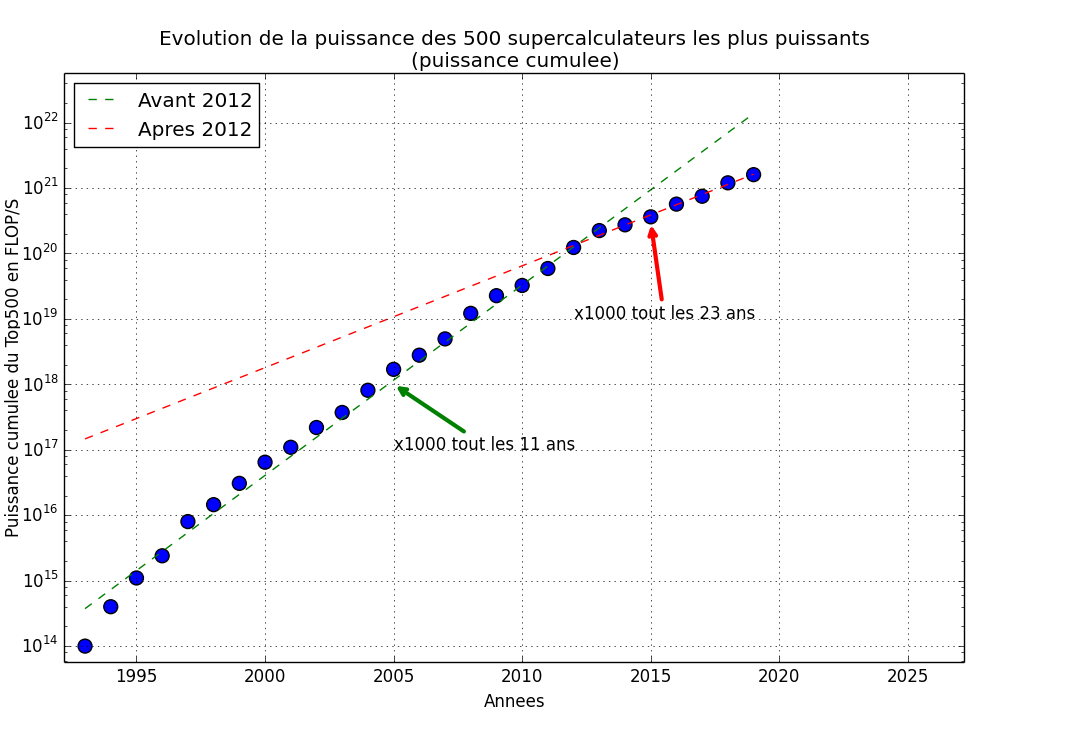
\includegraphics[width=14cm]{images/top500_evolution.png}
            \caption{\label{fig:top500_evolution_intro} Évolution de la performance cumulée des 500 supercalculateurs les plus puissants au monde, mesurée en FLOPS à l'aide du benchmark HPL (\textbf{todo accronyme}).}
        \end{figure}
        
        Nous remarquons sur la \autoref{fig:top500_evolution_intro} que la performance des supercalculateurs a évolué d'un facteur 1000 tous les 11 ans pendant près de 20 ans. Durant cette période, les processeurs ont pu profiter de nombreuses évolutions technologiques : augmentation du nombre de transistors et de la fréquence des processeurs, augmentation du nombre de coeurs ou encore l'implémentation d'une hiérarchie mémoire accélérant les accès aux données.
        Pour atteindre une puissance d'un exaflops, nous pouvons ainsi nous demander s'il ne suffirait simplement d'attendre les prochaines générations de processeurs et d'augmenter le nombre de serveurs formant un supercalculateur. Malheureusement, nous constatons à partir de 2012 un ralentissement de l'évolution des performances des supercalculateurs. Il faudra maintenant attendre 23 ans pour voir leur performance évoluer du même facteur 1000.
        Ce ralentissement est dû à un ensemble de contrainte qu'il n'est plus possible d'éviter, dont les deux principales sont la fin de la validité de loi de Moore, qui prévoyait l'augmentation du nombre de transistors chaque année, et la fin de la loi de Dennard, qui assurait l'augmentation les fréquences de chaque nouvelle génération de processeur.  De plus, les systèmes mémoires et les capacités de traitement des processeurs ont évolué de façon inégale. Lorsque la performance calculatoire augmentait de 50\% chaque année, le débit mémoire n'augmentait que de 23\%. Ce déséquilibre entre ces deux parties fondamentales de l'architecture Von Neumann a donné naissance au mur de la mémoire. À cause de cette inégalité d'évolution, les supercalculateurs modernes ne parviennent à extraire qu'une fraction des performances théoriques des architectures. Celle-ci  est parfois inférieure à 10\% \textbf{todo citer [Can+10]}.
        
        En plus des freins présentés ci-dessus, de nombreux défis supplémentaires doivent être relevés afin de poursuivre le rythme d'évolution des performances des supercalculateurs. Plusieurs études \cite{Sutter2005b, bergman2008exascale, Lucas2014, HPE2016} prédisent depuis plusieurs années les principales difficultés rencontrées pour développer une plateforme exascale : l'efficacité énergétique, les technologies d'interconnexion et mémoires, la gestion des données, la résistance aux erreurs… 
        Le principal défi est celui de l'énergie. Avec les technologies actuelles, un supercalculateur exascale consommerait plusieurs centaines de mégawatts, équivalent à la consommation électrique d'une ville comme Antibes (75 875 habitants). Pour des raisons de coût et de faisabilité, l'objectif de l'industrie HPC est de construire une plateforme exascale consommant entre 20 et 30 MW. Le challenge est donc de construire une plateforme sept fois plus puissante que le supercalculateur le plus puissant actuel, tout en étant trois fois plus efficace énergétiquement. Le déplacement des données à l'intérieur (entre la mémoire et le processeur) et à l'extérieur (entre deux serveurs) sont les principales opérations consommatrices d'énergie. Cette consommation peut être en partie expliquée par la complexité des microarchitectures, mais aussi par les technologies d'interconnexion utilisées. Cette complexité due aux nombreuses améliorations qu'ont connues les processeurs (hiérarchies mémoire, pipeline, d'unité de préchargement mémoire) est aussi à l'origine de la difficulté des applications à extraire plus d'une fraction des performances théoriques disponibles.
        

    \subsection{Les opportunités}


        L'incapacité des technologies actuelles à réaliser efficacement des calculs et l'explosion du nombre de données à traiter nécessite de repenser les matériels utilisés et l'architecture des systèmes informatiques. Heureusement de nouvelles technologies sont développées et peuvent permettre à l'industrie d'implémenter cette vision du calcul extrême.
        La première opportunité vient du développement de nouvelles technologies mémoires permettant de combler la différence d'évolution de performance constatée entre les processeurs et les mémoires. La faiblesse des débits mémoires et la consommation électrique du système mémoire obligent les architectures à évoluer drastiquement. La première solution est de rapprocher ces espaces mémoire des zones de calculs en plaçant la mémoire sur les puces de calculs (On Package Memory) ou en réalisant les calculs directement en mémoire (In Memory Computing).  La seconde solution est de développer de nouvelles technologies mémoires afin de combler le trou séparant les caractéristiques des mémoires DRAM et des disques de stockage flash. Pour cela des technologies NVRAM (non-volatile RAM) sont développées en s'appuyant notamment sur de nouvelles technologies mémoires SCM (storage class memory).
        Afin d'améliorer le débit des bus mémoire et d'interconnexion, des technologies photoniques sont actuellement développées. La principale qualité de ces technologies est d'être indépendant de la distance et de permettre d'atteindre des débits élevés. Bien que la génération d'un signal optique ou électronique nécessite la même énergie, celle-ci n'évolue que faiblement avec la distance de communication. Le coût énergétique d'un accès mémoire local est alors proche de celui d'un accès distant. 
        Ces nouvelles technologies, associées aux méthodes de co-design, qui associent les utilisateurs et les fabricants, vont permettre de développer de nouvelles architectures ultra-optimisées pour certains algorithmes.  L'utilisation d'architectures hétérogènes dans une même plateforme a été démocratisée par l'utilisation massive des GPU et doit être poursuivie avec de nouvelles architectures très différentes de celles actuellement utilisées : les accélérateurs produits par Google (TPU), NEC (SX-Aurora), ou encore Pezy (PEZY-SC2). 
        Afin de faciliter l'intégration de ces nouvelles technologies (mémoires, processeurs) provenant de différents constructeurs, de nouveaux protocoles doivent être développés. Un tel protocole est en cour de développement et propose un protocole de communication très simplifié utilisant une sémantique mémoire \verb=load/store=. Nommé Gen-Z, ce protocole est développé par 70 des plus grandes sociétés des technologies de l'information (IT). Il permettra d'adresser un espace mémoire mille fois plus grand que notre espace numérique actuel et interconnecter 16 millions d'objets sur une même fabric. Les premières versions d'architecture Gen-Z permettront d'atteindre des débits mémoires de plusieurs téraoctets par seconde contre quelques centaines de gigaoctets actuellement.

\section{Travail de thèse}

    
    Pour subvenir au besoin de puissance grandissant et ne pouvant compter sur les anciens leviers à sa disposition, l'industrie doit utiliser de nouvelles technologies émergentes et revoir la conception des plateformes de calculs. Ces ruptures technologiques sont telles, qu'elles permettront de faire des sauts de performance de plusieurs facteurs (10, 100 voir 1000).

    
    \subsection{Problématique}
    
        Grâce à Gen-Z et aux nouvelles technologies présentées précédemment, de nombreuses architectures vont être développées et seront très différentes de celles que nous utilisons actuellement (processeurs x86, GPU). Ces processeurs seront alors très efficaces pour l'exécution de certains types d'opérations et d'algorithmes. Afin de répondre aux besoins de performances supplémentaires et relever le défi de l'efficacité énergétique, il est nécessaire d'utiliser les architectures les plus adaptées pour l'exécution d'une application. Pour ce faire, trois tâches principales doivent être réalisées :
        \begin{enumerate}
            \item La première tâche est de caractériser l'ensemble de ces architectures pour trouver leurs forces et leurs faiblesses: débit et latence mémoire, capacité calculatoire, performance du système mémoire pour certains motifs d'accès. Ces nouvelles architectures pouvant être très différentes de celles que nous utilisons actuellement, il est indispensable de disposer d'un ensemble d'outils permettant de les caractériser pour différents types d'algorithmes.
        
            \item La deuxième tâche consiste à modéliser les performances d'une application pour en connaître ses besoins (débit et/ou latence mémoire, calcul vectoriel, système d'interconnexion, stockage…). Les gains de performance ne viendront pas seulement de l'utilisation d'accélérateurs puissants, mais de leur diversité et de la capacité des programmeurs à bien les utiliser. Pour une même application, plusieurs zones de code prenant une part importante dans son exécution peuvent avoir des besoins différents. Il est ainsi nécessaire de pouvoir identifier ces zones et de les modéliser indépendamment. 
        
            \item La troisième tâche est de sélectionner les architectures adéquates pour une application et adapter le code pour permettre son exécution. Il est ensuite nécessaire de pouvoir mesurer les performances de l'application et d'appliquer les optimisations adaptées pour obtenir une part significative de la performance théorique.
        \end{enumerate}
    
    \subsection{Travaux existants}
    
        Afin de répondre aux tâches présentées ci-dessus, les programmeurs doivent alors avoir à leur disposition un ensemble d'outils permettant de caractériser le comportement des architectures et d'étudier la performance de leurs applications lors de l'exécution.
        
        
        \subsubsection{Caractérisation des architectures}
            
            Afin de caractériser les architectures et de mesurer les performances atteignables par la microarchitecture, il est courant d'utiliser des benchmarks. En informatique, un benchmark est un code, ou un ensemble de codes, permettant de mesurer la performance d'une solution et d'en vérifier ses fonctionnalités. Dans ce travail de thèse, nous nous intéressons à la caractérisation de deux composants fondamentaux des processeurs utilisés en HPC : la hiérarchie mémoire et les unités de calcul vectorielles. 
            
            \paragraph{Caractérisation du système mémoire} 
            
                Le système mémoire étant le goulot d'étranglement principal des performances des applications, de nombreux travaux ont été menés pour aider à sa caractérisation. Le plus utilisé d'entre eux est le benchmark STREAM \cite{McCalpin1995}. Ce code utilise 4 noyaux de calculs différents pour mesurer le débit mémoire atteignable par une architecture. Pour cela, un tableau de nombres aléatoires stocké en mémoire est accédé par des instructions de lecture/écriture pour réaliser 4 opérations : copy, scale, add, triad. La simplicité de ces codes permet souvent d'atteindre les débits maximaux du bus mémoire et fait de STREAM un benchmark de référence. Un autre benchmark largement utilisé dans l'industrie est celui de Lmbench \cite{Staelin2004}. Lmbench est une suite de microbenchmarks utilisée pour mesurer la latence et le débit atteignable par un cœur pour différentes opérations : accès mémoire, ouverture de fichier, création de pipe. Il permet aussi de trouver certaines caractéristiques de la microarchitecture comme la taille d'une ligne de cache ou de celle de la TLB \textbf{todo TLB}.
                
                De nombreuses applications utilisent des accès mémoires réalisant des sauts d'adresses (stride) de taille constante. Par exemple, le parcours d'un tableau d'objet pour accéder à un certain champ ou le parcours d'une matrice (en ligne ou en colonne). Pour accélérer ces accès, l'unité de préchargement mémoire peut anticiper les prochaines adresses accédées en comprenant le motif d'accès utilisé et commencer leur chargement avant qu'elles ne soient accédées. Pour des applications utilisant ce type d'accès par saut, il est primordial que ce composant fonctionne correctement pour réduire au maximum le manque d'une donnée dans le cache lors de son accès.
                Au moment de la réalisation de ce travail de thèse, il n'existe à notre connaissance aucun benchmark permettant de caractériser l'architecture pour ce type d'accès. Le benchmark s'approchant le plus de cet objectif est celui de Saavedra  \cite{Saavedra1995}.  Il utilise une taille de saut fixée au début de l'exécution pour accéder à un jeu de données. La taille de ce dernier doit être un multiple d'une puissance de 2 et ne permet pas de dépasser la taille du dernier niveau de cache. Le problème d'une telle approche est de vouloir mesurer tous les niveaux de la hiérarchie simultanément. Les mesures peuvent alors être influencées par différents paramètres de différents niveaux de caches.
        
            \paragraph{Caractérisation des unités de calculs vectorielles}
            
                La majorité des applications utilisées en HPC exécutent des \gls{FLOP}. Ces instructions sont exécutées par un matériel spécialisé nommé \gls{ALU}. La capacité des ALU à exécuter plusieurs instructions vectorielles par cycle est alors primordiale pour la bonne performance des applications. La littérature dénombre plusieurs benchmark couramment utilisés pour mesurer la performance de calcul des processeurs. Le benchmark HPL  \cite{Dongarra2003} a été développé pour caractériser la microarchitecture d'un processeur lors de la résolution de problèmes algébriques. Ce code permet aujourd'hui de mesurer et classer les supercalculateurs dans le classement du Top500. Le benchmark HPL n'étant pas représentatif d'applications réelles, un ensemble de codes a été rassemblé pour améliorer la caractérisation des supercalculateurs. Nommé HPCG \cite{Dongarra2013}, cet ensemble de codes permet de couvrir plusieurs motifs de communication et de calculs. Les versions récentes du Top500 publient pour certains supercalculateurs la performance obtenue sur le benchmark HPCG. Nous pouvons aussi citer le benchmark HPCC \cite{Luszczek2006} qui est une suite de 6 benchmarks contenant notamment HPL et STREAM. Un seul exécutable est généré pour l'ensemble de la suite permettant d'éviter l'utilisation de certaines optimisations pour un code particulier (pages larges, réglage BIOS…). 

                Nous constatons le manque d'un outil permettant de valider précisément les performances des unités de calculs. Un tel outil permettrait en effet d'étudier le comportement précis des ALU : le nombre d'instructions par cycle pour différentes opérations vectorielles, la possibilité de combiner des instructions différentes, la sensibilité aux chaînes de dépendances.
                
                
        \subsubsection{Suivi de performance des applications}
        
            Le deuxième aspect de nos recherches concerne le suivi de performances des applications. L'objectif de celui-ci est de récolter des informations concernant l'application ou le système. Ces informations peuvent être obtenues en instrumentant le code (manuellement ou grâce au compilateur) ou en récupérant certaines informations de l'architecture. Pour cela, les processeurs possèdent des registres (compteurs) qui permettent de compter des événements (matériels ou logiciels) avec un faible impact sur l'application exécutée. Chaque famille de processeurs possède un jeu différent de compteurs matériels pouvant avoir des noms différents, rendant leur programmation difficile. Afin de faciliter leur programmation, des interfaces comme \verb=PAPI= \cite{Browne2000} et \verb=Perf Events= \cite{Weaver2013} ont été développées. Celles-ci permettent de développer des outils sans se préoccuper de l'implémentation matérielle des compteurs facilitant ainsi la portabilité des outils. Nous pouvons notamment citer les outils d'Intel (\verb=VTune=), de Linux (\verb=perf=) ou encore ceux développés au Barcelona Supercomputing Center (\verb=Extrae= \cite{Rodriguez}, \verb=Paraver= \cite{Pillet1995} et \verb=Dymemas= \cite{Labarta1997}).
            
            Afin de répondre aux différentes tâches de la problématique traitée dans ce travail de thèse, deux outils principaux sont nécessaires. 
            Le premier doit permettre de suivre l'activité du bus mémoire. Ce bus est une ressource critique des architectures modernes, rendant sa bonne utilisation indispensable. Il est donc nécessaire de posséder un outil permettant de suivre l'état du trafic sur ce bus. Pour cela, des outils existent, mais sont soit propriétaires, soit trop complexes pour être facilement installés sur des architectures novatrices. 
            Un second outil doit être capable d'extraire les zones de codes les plus intéressantes à porter sur ces nouvelles architectures. Les supercalculateurs seront hétérogènes et utiliseront plusieurs accélérateurs différents adaptés à certaines fonctions. Une même application pourra alors faire appel à plusieurs d'entre eux. Il est donc nécessaire de posséder un outil permettant de caractériser les différentes fonctions d'une même application en extrayant ces zones de codes et en les caractérisant.  Ce même outil pourrait alors aussi être utilisé pour comprendre les performances de l'application et appliquer les optimisations adéquates. 

\section{Contributions et plan du manuscrit}
    
    L'industrie va faire face à une multitude de révolutions technologiques, et les utilisateurs de supercalculateur doivent se préparer à ces changements profonds pour pouvoir les exploiter au maximum. Contrairement aux évolutions précédentes où il suffisait d'installer un nouveau processeur ou d'ajouter des barrettes mémoires, il faut repenser entièrement notre façon d'appréhender les architectures des supercalculateurs et adapter les algorithmes qui y seront exécutés. Cependant, en l'absence de méthode de caractérisation fine de la performance des codes, ces architectures innovantes sont potentiellement condamnées puisque peu d'experts savent les valoriser. En effet, la loi de Moore a permis d'assurer une évolution constante des processeurs, laissant le domaine de l'analyse et l'optimisation des codes en second plan. Ainsi, nous avons constaté à travers de nombreuses rencontres avec les utilisateurs, mais aussi par les expériences internes à HPE, le manque d'outils et de connaissances nécessaires à la réalisation de ce travail.
    
    \subsection{Contributions}
        
        Afin de pouvoir profiter de ces nouvelles technologies, nous proposons dans ce travail une méthodologie en 5 étapes permettant de modéliser les performances d'une application, de les projeter sur de nouvelles architectures et d'en extraire la performance maximale. Pour chaque étape, nous avons développé et sélectionné des outils permettant de répondre aux challenges présentés et qui respectent certains critères :
        \begin{itemize}
            \item Les sources de l'outil doivent être disponibles pour permettre de les adapter à des architectures différentes et pour développer une communauté d'utilisateurs autour de ces sujets,
            \item Les outils doivent être simples, ne cherchant pas à répondre à une multitude de questions qui rendent difficile leur portabilité, mais aussi les conclusions pouvant être tirées des résultats obtenus,
            \item Les outils doivent permettre d'analyser des applications HPC dont l'exécution peut durer plusieurs heures. Il faut aussi réduire au maximum la nécessité de posséder des droits spéciaux (root) pour les utiliser, ce dernier étant rarement disponible pour les utilisateurs de supercalculateurs.
        \end{itemize}
        
        Les outils n'ont pas vocation d'automatiser entièrement les tâches du programmeur. La puissance de ces outils vient de leur utilisation complémentaire. Nous espérons qu'en réduisant la complexité de l'outillage, l'adoption des outils auprès des programmeurs sera plus grande. Nous avons développé un outil lorsqu'aucun programme existant ne pouvait être utilisé pour la réalisation d'une étape de la méthodologie, ou qu'il ne respectait pas les critères énoncés ci-dessus. Les principales contributions de cette thèse sont :
        \begin{enumerate}

            \item \textbf{Un benchmark mémoire} – \verb=DML_MEM= : ce benchmark permet de mesurer le débit mémoire en réalisant des accès dans un tableau avec des motifs de sauts (strides). La taille du tableau et des sauts peut varier et permet de caractériser les différents niveaux de la hiérarchie mémoire. Cet outil est utile pour caractériser une nouvelle architecture, mais peut aussi être utilisé lors du design d'un nouveau processeur pour vérifier le bon fonctionnement du préchargement mémoire.
            
            \item \textbf{Un benchmark d'unité arithmétique et logique (ALU)} – \verb|Kernel Generator| : ce générateur permet de caractériser finement les performances des unités arithmétiques et logiques (ALU). Pour cela, il génère un benchmark assembleur en utilisant des instructions vectorielles de taille différentes (SSE, AVX2, AVX-512). L'utilisateur peut alors choisir le type d'opération à exécuter (addition, multiplication, FMA) et la précision (simple, double). La partie du benchmark mesurée ne contient que des instructions de calculs et permet de mesurer très précisément la performance atteignable pas le processeur (souvent proche ou égale à la performance théorique).
                        
            \item \textbf{Un outil de suivi d'activité du bus mémoire} -  \verb=YAMB= : cet outil est basé sur l'interface perf et permet de mesurer le trafic mémoire sur le bus en discernant les lectures et les écritures. YAMB établit le profil de chaque contrôleur mémoire en mesurant le nombre de transactions (lecture et écriture) ainsi que le nombre d'accès manqués (miss) dans le dernier niveau de cache (LLC). Pour corréler l'activité du bus avec les parties du code qui en sont responsables, le graphique peut facilement être annoté en utilisant une API C/C++/Fortran, appelée directement depuis le code source.
            
            \item \textbf{Un outil extraction des \glspl{kernel}} – \verb=Oprofile++=: cet outil permet de désassembler le code d'une application, d'extraire les boucles critiques d'en mesurer la performance. Oprofile++ est basé sur les outils Oprofile et Objdump. Il permet dans un premier temps de relier le profile aux instructions assembleurs exécutées. Ensuite, il s'occupe d'extraire les boucles critiques et de mesurer le nombre d'instructions exécuté chaque cycle (IPC). Il est ensuite possible de quantifier des opportunités d'amélioration, mais aussi de prédire la performance en fonction d'une amélioration du matériel ou du logiciel.
            
            \item \textbf{Une méthodologie pour le portage et l'optimisation} : Afin d'utiliser de façon efficace les outils sélectionnés et développés, nous avons décrit une méthodologie en 5 étapes. Celle-ci permet de sélectionner la meilleure architecture pour une application donnée et d'en extraire le maximum de performance.
        
        \end{enumerate}
        
    \subsection{Plan du manuscrit}
    
        Cette thèse propose une étude étendue du domaine du HPC pour comprendre et contribuer à l'élaboration des prochaines générations de plateformes de calculs. Pour cela, le manuscrit suit la structure suivante :
        
        \begin{itemize}
        
            \item Le \autoref{chap:hpc} introduit le domaine du calcul haute performance en étudiant ses origines et en présentant leur architecture actuelle et les moyens employés pour les programmer. Nous discutons ensuite de leur performance en étudiant l'évolution du classement du Top500 et nous expliquons notamment les principaux freins qui empêchent de construire des plateformes toujours plus puissantes avec les méthodes actuelles. Afin d'y parvenir, nous présentons les principales opportunités technologiques actuellement développées qui vont nous permettre de repenser l'architecture des plateformes. La fin de ce chapitre s'intéresse plus précisément à la caractérisation des microarchitectures et à l'analyse de performance d'applications.
        
            \item Le \autoref{chap:dev} présente les principaux outils développés durant ces travaux de thèse. Nous discutons des motivations et des critères de développement qui nous ont conduits à développer deux benchmarks et deux outils d'analyse de performance.
        
            \item Le \autoref{chap:methodo} présente en détail la méthodologie élaborée et utilisée pour caractériser et choisir une architecture pour une application donnée. Nous utilisons l'analyse du benchmark STREAM et d'un processeur Intel Skylake pour illustrer chacune des 5 étapes.
        
            \item Afin de permettre la réalisation des différents codes développés, l'étude approfondie des différentes évolutions technologiques des processeurs et des techniques de suivi de performances sont présentées dans deux annexes de ce manuscrit:
            \begin{itemize}
                \item L'\aref{annexe:CHAPITRE_ARCHITECTURE} couvre l'origine et l'évolution de la microarchitecture des processeurs. Nous présentons les fonctionnalités clés des processeurs modernes qu'il est nécessaire de connaître pour comprendre la performance des applications: pipeline, instructions vectorielles, etc. Nous étudions plus précisément la hiérarchie mémoire qui est la ressource critique de nombreuses applications. 
                
                \item L'\aref{annexe:hardware_counter} présente les compteurs matériels. Ces registres spéciaux du processeur permettent de suivre l'exécution d'une application en mesurant le nombre d'évènements logiciels et matériels. La programmation des compteurs est très difficile et nécessite le recours à des codes bas niveaux. Plusieurs méthodes peuvent alors être employées et demandent une bonne expérience pour être mise en oeuvre.
            \end{itemize}
            Nous faisons référence à ces deux annexes lorsque les concepts qui y sont étudiés sont utilisés dans le manuscrit.
        
        \end{itemize}